\documentclass[a4paper,12pt]{article}

\usepackage{comment}
\usepackage{supertabular}
\usepackage{graphics}
\usepackage{color,soul}
\usepackage{booktabs}
\usepackage{paralist}
\usepackage{algorithmicx}
\usepackage{algorithm}
\usepackage[noend]{algpseudocode}
\usepackage{booktabs}
\usepackage{hvfloat}
\usepackage{comment}
\usepackage{chngpage}
\usepackage{url}
\usepackage[utf8]{inputenc}
\usepackage[table,dvipsnames]{xcolor}
\usepackage[a4paper,pdftex,hmargin=0.75in,vmargin={1.1in,0.6in},head=75pt,foot=45pt, left=2.5cm, right=2.5cm, includefoot, footskip=60pt]{geometry}
\usepackage{lipsum}
\usepackage{afterpage}
\usepackage{xcolor}
\usepackage{tabularx}
\usepackage{wallpaper}
\usepackage{adjustbox}
\usepackage[normalem]{ulem}
\useunder{\uline}{\ul}{}
\usepackage{rotating}
\usepackage{parskip}
\usepackage{listings}
\lstset{language=C,breaklines=true}
\usepackage[english]{babel}
\usepackage{amsmath}
\usepackage{amsfonts}
\usepackage{amssymb}
\usepackage[justification=centering]{caption}
\usepackage{fontenc}
\usepackage[colorlinks=true]{hyperref}
\usepackage{multicol}
\usepackage{multirow}
\usepackage{array}
\usepackage{relsize}
\usepackage{subcaption}
\usepackage{caption}
\usepackage{tcolorbox}
\usepackage{lscape}
\usepackage{lastpage}
\usepackage{acro}
\setlength{\headsep}{1.5cm}
\usepackage[toc,page]{appendix}
\usepackage[nottoc]{tocbibind} % for show references in toc
\usepackage{pgfgantt}
\frenchspacing
%\usepackage{svg}
%\usepackage{showframe}% for show page layout

\colorlet{punct}{red!60!black}
\definecolor{background}{HTML}{EEEEEE}
\definecolor{delim}{RGB}{20,105,176}
\colorlet{numb}{magenta!60!black}
\lstdefinelanguage{json}{
    basicstyle=\normalfont\ttfamily,
    numbers=left,
    numberstyle=\scriptsize,
    stepnumber=1,
    numbersep=8pt,
    showstringspaces=false,
    breaklines=true,
    frame=lines,
    backgroundcolor=\color{background},
    literate=
     *{0}{{{\color{numb}0}}}{1}
      {1}{{{\color{numb}1}}}{1}
      {2}{{{\color{numb}2}}}{1}
      {3}{{{\color{numb}3}}}{1}
      {4}{{{\color{numb}4}}}{1}
      {5}{{{\color{numb}5}}}{1}
      {6}{{{\color{numb}6}}}{1}
      {7}{{{\color{numb}7}}}{1}
      {8}{{{\color{numb}8}}}{1}
      {9}{{{\color{numb}9}}}{1}
      {:}{{{\color{punct}{:}}}}{1}
      {,}{{{\color{punct}{,}}}}{1}
      {\{}{{{\color{delim}{\{}}}}{1}
      {\}}{{{\color{delim}{\}}}}}{1}
      {[}{{{\color{delim}{[}}}}{1}
      {]}{{{\color{delim}{]}}}}{1},
}

%RBG FFD33E / C95D40
\definecolor{upcorange}{HTML}{FFD33E}
\hypersetup{allcolors=black}

% probably a good idea for the nomenclature entries:
\acsetup{first-style=short}

%%%% PAGE STYLE %%%%%
\usepackage{fancyhdr}
\pagestyle{fancy}
\fancyhf{}
\lhead{
\includegraphics[height=1.2cm]{img/logos/upclogo.png}}
\rhead{
\includegraphics[height=1.2cm]{img/logos/logo_telecos.png}}
\rfoot{\thepage{}}

\renewcommand{\footrulewidth}{0.4pt}
%\futurelet\TMPfootrule\def\footrule{{\color{upcorange}\TMPfootrule}}
\futurelet\TMPfootrule\def\footrule{{\color{gray!80}\TMPfootrule}}
\renewcommand{\headrulewidth}{0.4pt}
\renewcommand{\headrule}{\hbox to\headwidth{%
%\color{upcorange}\leaders\hrule height \headrulewidth\hfill}}
\color{gray!80}\leaders\hrule height \headrulewidth\hfill}}
%\renewcommand*\ShowFrameColor{\color{red}}

% class `abbrev': abbreviations:
\DeclareAcronym{EU}{
  short = EU ,
  long  = European Union ,
  tag = abbrev % class
}

\DeclareAcronym{ETSETB}{
  short = ETSETB ,
  long  = Escola Tècnica Superior d'Enginyeria de Telecomunicació de Barcelona ,
  % long = Barcelona School of Telecommunications Engeneering ,
  tag = abbrev % class
}



\begin{document}

%%% COVER %%%
\fancypagestyle{alim}{\fancyhf{}\renewcommand{\headrulewidth}{0pt}
\cfoot{
\includegraphics[height=2.2cm]{img/logos/logo_telecos.png}}
}
\thispagestyle{empty}
\begin{center}
{\sffamily 
\resizebox{0.8\textwidth}{!}{
\includegraphics{img/logos/upc_completo+telecos.png}}\\
\vspace{1cm}
{\Huge Design of a diversity enforcement module for safety critical processing systems}\\
\vspace{0.5cm}
{\color{black}\hrule height 1pt}
\vspace{1cm}
{\large{Master Thesis\\
submitted to the Faculty of the \\
Escola T\`ecnica d'Enginyeria de Telecomunicaci\'o de Barcelona \\
Universitat Polit\`ecnica de Catalunya \\
by\\
\vspace{0.4cm}
Francisco Bas Jalón}}

\nocite{*} % only if you no use \cite{}

\vspace{1.5cm}

{In partial fulfillment\\
of the requirements for the master in\\
\textit{Electronic} \textbf{ENGINEERING}}

\vspace{2cm}

{{Advisor: Francesc Moll Echeto}} \\
{{Advisor: Jaume Abella Ferrer}} \\
{{Barcelona, Date 02/07/2022}}
\thispagestyle{alim}
}

%%% INDEX %%%
\end{center}
\newpage
\tableofcontents

%%% LISTS %%%
\newpage
\listoffigures
\lstlistoflistings
\listoftables

%%% REVISION %%%
\newpage
\section*{Revision history and approval record}

\selectlanguage{english}
\foreignlanguage{english}

\begin{center}
\tablefirsthead{}
\tablehead{}
\tabletail{}
\tablelasttail{}
\begin{supertabular}{|m{1.908cm}|m{2.398cm}|m{11.489cm}|}
\hline
\textbf{Revision} &
\textbf{Date} &
\textbf{Purpose}\\\hline
0 &
dd/mm/yyyy &
Document \ creation\\\hline
1 &
dd/mm/yyyy &
Document \ revision\\\hline
~
 &
~
 &
~
\\\hline
~
 &
~
 &
~
\\\hline
~
 &
~
 &
~
\\\hline
\end{supertabular}
\end{center}

\bigskip

{\selectlanguage{english}
DOCUMENT DISTRIBUTION LIST}

\begin{center}
\tablefirsthead{}
\tablehead{}
\tabletail{}
\tablelasttail{}
\begin{supertabular}{|m{8.205cm}|m{7.589cm}|}
\hline
\textbf{\ Name} &
\textbf{\ e-mail}\\\hline
\ [Student name] &
~
\\\hline
[Project Supervisor 1] &
~
\\\hline
[Project Supervisor 2] &
~
\\\hline
~
 &
~
\\\hline
~
 &
~
\\\hline
~
 &
~
\\\hline
\end{supertabular}
\end{center}

\bigskip

\begin{center}
\tablefirsthead{}
\tablehead{}
\tabletail{}
\tablelasttail{}
\begin{supertabular}{|m{1.925cm}|m{6.1990004cm}|m{1.901cm}|m{5.6140003cm}|}
\hline
\multicolumn{2}{|m{8.324cm}|}{ Written by:} &
\multicolumn{2}{m{7.715cm}|}{ Reviewed and approved by:}\\\hline
 Date &
 dd/mm/yyyy &
 Date &
 dd/mm/yyyy\\\hline
 Name &
 Xxxxxxx yyyyyyy &
 Name &
 Zzzzzzz \ Wwwwwww\\\hline
 Position &
 Project Author &
 Position &
 Project Supervisor\\\hline
\end{supertabular}
\end{center}


%%% ABSTRACT %%%
\clearpage
\newpage
\section*{Abstract}

Safety-critical systems must adhere to specific functional safety standards describing the development process for those systems. One key requirement is the ability to avoid a single fault from causing a system failure, or in other words, avoiding Common Cause Failures (CCFs). Redundancy is a usual solution against CCFs. However, some specific CCFs may affect redundant components identically (e.g., voltage droops, clock interferences), hence potentially leading to identical errors that may go unnoticed and cause a failure.
Diversity is often deployed along with redundancy to avoid also those CCFs. In the particular case of computing elements (e.g., cores), this is usually realized with some form of lockstep execution where two identical cores execute the same software, but with some time shift among them (aka staggering). Therefore, both cores have different state at any point in time and faults affecting both cores lead to different errors, which can be detected by comparing the outputs.
Unfortunately, existing solutions have some non-negligible costs: (i) hardware-only solutions hide half of the cores making them non-user visible, hence halving platform performance even for non-critical tasks. Conversely, (ii) software-only solutions are much more flexible but impose the use of a third core to run the lockstep monitor, and require large staggering which has significant impact in performance for short programs.

This thesis devises a new solution aiming at combining the advantages of existing solutions. Our proposal, a hardware diversity-enforcement module (referred to as SafeDE), is an efficient hardware realization of the software monitor. Therefore, it does not hide any core to the end user, it does not require a third core for monitoring purposes, and allows operating with tiny staggering (e.g., few tens of cycles instead of hundreds of thousands as required for the software-only solution). 

We implement and integrate SafeDE in a space multicore prototype in an FPGA and validate that it effectively achieves its requirements with negligible hardware costs. Moreover, this work has already led to the publication of two peer-reviewed articles in especialized conferences and journals.

%{Every copy of the thesis must have an abstract. An abstract must provide a concise summary of the thesis. In style, the
%abstract should be a miniature version of the thesis: short introduction, a summary of the results, conclusions or main
%arguments presented in the thesis. The abstract may not exceed 150 words for a Degree’s thesis.}

\clearpage
\newpage
\section{Introduction}




\subsection{Context and Objectives}

High-performance multicores are needed to deliver the increasing performance demands of highly-automated and autonomous systems in automotive, avionics and space, among other domains. However, performance demands come along with safety requirements in those domains, as dictated in corresponding functional safety standards (e.g., ISO26262 in automotive~\cite{ISO26262}).
One such requirement for high-integrity systems consists of deploying redundancy to detect errors, but avoiding the unacceptable risk (aka unreasonable risk in ISO26262 terminology) of \emph{common cause failures} (CCFs), where a CCF stands for a failure caused by a single fault affecting all redundant components analogously. Note that CCFs relate to the effect, i.e. the failure, not to the source, i.e. the fault. Hence, CCFs could be caused, for instance, by a soft error affecting clock logic of two cores, or by a defect causing voltage sporadic droops. If such a single fault drives the redundant items (e.g. two cores running the same program redundantly) to the same error, so that it cannot be detected by comparing the results of the redundant items, then it is said that such fault induces a CCF.

CCFs are generally mitigated by using diverse redundancy~\cite{ClassicDiversity}, so that, even if a fault affects all redundant components (e.g., a voltage droop), since they have different state, potential errors differ and can be detected. Error correction codes (ECC) for storage, Cyclic Redundancy Coding (CRC) for communications, and lockstepping for computation are the most common solutions~\cite{alcaide2019software}. ECC and CRC build on generating a form of signature of the data protected, being such signature the result of applying some operations on the data. Hence, the signature and data have different length and different values (and hence, are diverse). If a fault, such a voltage droop, when reading, storing or transmitting data causes perturbations that lead to altered values read, written or transmitted, the likelihood of the signature matching the data tends to zero (e.g., chances of matching may easily be $\frac{1}{2^K}$ for $K$-bit signatures), and hence the error is, at least, detected.
Nevertheless, the focus of this thesis is lockstep execution for computation~\cite{STlockstep,infineon2012aurix,iturbe2019arm,paper1}. 

Lockstep execution (hardware-only) builds upon identical redundant cores running the same software with some staggering -- i.e. the head core runs $N$ cycles ahead of the trail one. Such staggering makes that, at any point in time, the state and activity across redundant cores is dissimilar, and hence, diverse redundancy is attained as long as some staggering holds.
In lockstep execution, one of the cores effectively sends and receives external signals (e.g., load/store data, interrupts, etc.). The outputs of the other core are just used for comparison for error detection reasons. However, in such a scheme only one core is visible at user level, thus not allowing to use both cores to run independent tasks if lockstep execution is not needed.

A light-weight lockstep execution scheme has been recently proposed to overcome the limitations of regular hardware-only lockstepping~\cite{alcaide2020software}. Such solution builds on software redundancy (i.e., the task is run redundantly from the software layers), and on a software monitor enforcing sufficient staggering between redundant processes. However, due to the slow software monitoring loop, staggering is significant (e.g., 100$\mu$s - 1ms), which imposes a performance loss as significant as such staggering (as opposed to the hardware-only solution whose staggering is few cycles), and requires an additional core to run the monitor periodically.

The objectives of this thesis consist of devising, integrating in an SoC, and evaluating a hardware module that achieves diverse redundancy for computation, but overcoming the main disadvantages of hardware-only lockstep execution and light-weight software-only lockstep execution. 
%In particular, we aim at designing and evaluating the hardware counterpart of the software-only solution. 
Therefore, this thesis presents SafeDE, a \underline{D}iversity \underline{E}nforcement hardware module overcoming the limitations of the previous two schemes. In particular, SafeDE implements the light-weight lockstep execution scheme, but with a hardware monitor (SafeDE module) rather than a software module, hence allowing for few-cycles staggering and not needing any additional core to run any monitor software. Moreover, the integration of SafeDE does not require modifying the cores being monitored, hence being a lowly intrusive solution.
The main contributions of this work are as follows:
\begin{itemize}
\item We present SafeDE, the monitoring module to enable lowly-intrusive diverse redundancy with a flexible scheme that can be enabled or disabled at convenience. We further detail how to extend it to arbitrary redundancy (e.g., with 3 or more cores instead of only 2).
\item We implement it at VHDL in two SoCs for the space domain based on CAES Gaisler's NOEL-V cores~\cite{gomez2020risc,SELENEgit}, and provide details on its bare metal and Linux integrations.
\item We assess SafeDE's performance and area overheads, as well as effectiveness through a fault injection campaign.
\end{itemize}



\subsection{Requirements and Specifications}

This work aims at developing SafeDE, a hardware module providing support for light-weight diverse redundancy. The requirements for such module are as follows:
\begin{itemize}
\item It must allow cores executing redundant tasks have a staggering much lower than that needed by the software-only solution. In general, a staggering in the order of some hundreds (or even few thousands) of cycles would be considered low enough. 
\begin{itemize}
\item As we show later in this document, we achieved this goal by setting a staggering of 20 instructions which, in practice, execute in some tens of cycles.
\end{itemize}
\item The module can be enabled and disabled by the end user within its applications so that lockstep execution is used only when needed. 
\begin{itemize}
\item As we show later in this document, activation and deactivation of the module is achieved by setting/resetting specific registers of the module that can be controlled by the end user from its own applications.
\end{itemize}
\item Hardware costs, typically in terms of area, must be low (e.g., below 5\% of the overall SoC).
\begin{itemize}
\item As we show later in this document, the cost in the FPGA implementation of the SoC is well below 1\% to make 2 cores operate in lockstep mode. If further cores are incorporated into the SoC, other SafeDE module instances should be added (one per pair of cores). Hence, the relative cost of the SafeDE module is expected to remain quite constant in relative terms with respect to the overall SoC.
\end{itemize}
\end{itemize}


\subsection{Methods, Procedures and Previous Work}
Since the goal was implementing SafeDE in the context of existing SoCs~\cite{gomez2020risc,SELENEgit}, and the software counterpart of SafeDE already existed~\cite{alcaide2020software}, those SoCs and software-only solution shaped the methodology. In particular, the software-only solution determines that the input to the SafeDE module is the instruction count of the cores running tasks redundantly, and the output is a signal capable of stalling one of the cores. The particular SoC, and its specific cores, determine the signals that need being exported from those IPs so that SafeDE can monitor execution progress and stall the corresponding core whenever there is risk of losing diversity.

Since the design has been prototyped in a FPGA, the toolflow used in the project where those SoCs were designed and enhanced has been inherited for this work. 

Finally, for validation purposes, SafeDE has been implemented including a number of debug features capable of counting how many times diversity is lost, how many instructions one core is ahead of the other, and the like. Such information allowed validating the correctness and efficiency of the implementation providing factual evidence of the actual staggering achieved across redundant cores. Tests were conducted with a wide variety of relevant benchmarks on a baremetal setup to validate the implementation.

Regarding previous work, we build on the software-only solution proposed by Alcaide et al.~\cite{alcaide2020software}. Such solution is described in more detail in Section~\ref{section:software_light_lockstep}, but essentially consists of a software monitor (a program) running periodically and reading the instruction count registers of two cores executing a program redundantly. If the staggering among them is regarded as too low, then the monitor send a stall signal to the core behind (trail core), and whenever the other core (head core) is ahead enough, the execution in the trail core is resumed by the monitor. In our case, the monitor is implemented as a hardware module (SafeDE), the monitoring frequency is every cycle, and the staggering needed much lower due to the higher frequency to check the staggering and the almost immediate control to stall the trail core.


\subsection{Work Plan and Deviations}
We had the opportunity of starting this work in the context of a European project well ahead of the time of starting the TFM. Hence, no specific work plan was stablished and execution of the work was based on the same flow used for other components of the SoC, and monitored with weekly meetings plus ad-hoc meetings to discuss unforeseen cases. As a result, the work was complete before the official start of the TFM and published in the two publications indicated in the following subsection, and the only part remaining was the preparation of this document. 

For obvious reasons, since the work was executed timely, no deviation can be claimed to have occurred.


\subsection{Publications}

This work has led to the following two publications in especialized peer-reviewed conferences and journals:

\begin{itemize}
\item 
Francisco Bas, Sergi Alcaide, Ruben Lorenzo, Guillem Cabo, Guillermo Gil, Oriol Sala, Fabio Mazzocchetti, David Trilla, Jaume Abella.
\emph{SafeDE: a Flexible Diversity Enforcement Hardware Module for Light-lockstepping}. 
\textbf{IEEE 27th International Symposium on On-Line Testing and Robust System Design (IOLTS)}, 2021, pp. 1-7, doi: 10.1109/IOLTS52814.2021.9486715.

\item
Francisco Bas, Sergi Alcaide, Guillem Cabo, Pedro Benedicte, Jaume Abella.
\emph{SafeDE: A Low-Cost Hardware Solution to Enforce Diverse Redundancy in Multicores}.
\textbf{IEEE Transactions on Device and Materials Reliability}, vol. 22, no. 2, pp. 111-119, June 2022, doi: 10.1109/TDMR.2022.3156799.
\end{itemize}

Moreover, we have also developed a complementary module (SafeDM) measuring diversity to allow end users choose whether they want to enforce diverse redundancy at hardware level with SafeDE, or just let software run unconstrainedly and monitor diversity with SafeDM so that, upon loss of diversity, system level measures are taken.
This other module has been also published (it is not part of this master thesis):

\begin{itemize}
\item 
Francisco Bas, Pedro Benedicte, Sergi Alcaide, Guillem Cabo, Fabio Mazzocchetti, Jaume Abella.
\emph{SafeDM: a Hardware Diversity Monitor for Redundant Execution on Non-Lockstepped Cores}.
\textbf{IEEE 25th Design, Automation and Test in Europe Conference and Exhibition (DATE)}, 2022, pp. 358-363, \linebreak doi: 10.23919/DATE54114.2022.9774540.
\end{itemize}

Also, a comparison between the different solutions (SafeDE, software-only and SafeDM) has also been published, yet the paper is still to appear:
\begin{itemize}
\item 
Ramon Canal, Francisco Bas, Sergi Alcaide, Guillem Cabo, Pedro Benedicte, Francisco Fuentes, Feng Chang, Ilham Lasfar, Jaume Abella.
\emph{SafeDX: Standalone Modules Providing Diverse Redundancy for Safety-Critical Applications}.
\textbf{22nd International Conference on Embedded Computer Systems: Architectures, Modeling and Simulation (SAMOS)}. Invited to the special session on Reports from research projects - Digital services and platforms: Application areas automotive industry, energy, agriculture, healthcare and industry 4.0 workshop. 2022.
\end{itemize}




%%% StateOfTheArt %%%
\clearpage
\newpage
\section{Background and state of the art}

\subsection{Faults, Failures and Errors}

During this thesis, the common terminology in fault-tolerant systems \cite{AlgirdasAvizienis2004} is employed:

Any electronic system delivers a service that the user of that system perceives. This service comprises all the external states of the system. A service \textbf{failure} or \textbf{system failure} occurs when the delivered service (i.e., one or more external states) deviates from the correct service state. The correct service is defined by the functional specification of the system. A failure in safety-critical systems can endanger lives or produce high economic losses. Thus, the main goal of safety-critical systems is to minimize the probability of a system failure.

The deviation between the correct internal or external state and the real state is called an \textbf{error}. The cause of an error is called a fault. Thus, a \textbf{fault} is a defect within the system. A fault first causes an error in one of the components that form the system, altering the system's internal state. If this error propagates to the system's output altering the external state and the service provided, we will say that the error led the system to a failure. However, not all faults produce errors and not all the errors reach the external estate of the system producing a failure.  

For instance, consider a two-inputs AND gate inside a system. If one input of the gate is '1' and the other is '0', the expected output will also be '0'. In this scenario, a fault that flips the logic driving the input with value '0' to a '1' will modify the AND gate output to '1', producing an error. However, if a fault flips the other input from '1' to '0', the output will still be '0', the expected value. 

Following the same logic, an AND gate, whose inputs are driven from two registers, one of them with an incorrect value (error), could correct the error preventing it from spreading to other registers and reaching the output of the system.

Faults can be classified into two main categories: \textbf{Systematic faults} that are related in a deterministic way to a certain cause and are avoidable by construction. These faults can be avoided by taking into account possible faults during the first step of the design or by investing enough resources into verification and validation processes \textcolor{red}{(examples....)}. \textbf{Random faults} that occur unpredictably following a probabilistic distribution and are unavoidable. This work focuses on Common Cause Faults (CCF), a particular type of random faults that will be explained later. \textcolor{red}{(examples....)}

\bigskip


\subsection{Safety Related Systems}

Safety-critical systems are those systems that need to work correctly because otherwise, a failure or malfunctioning could jeopardize people's life or health, produce losses in expensive equipment or cause environmental harm. For this reason, these systems must have mechanisms to lower the failure rates until they happen with a negligible likelihood. For instance, in the standards of the aircraft industry, an acceptable failure rate is $10^-9$ accidents per hour \cite{bowen2000ethics}.

Some errors, like systematic errors, can be found and corrected during the development process or mitigated by applying qualitative measures depending on the desired system integrity level SIL \textcolor{red}{citar libro??}. However, random faults could not be avoided and require special mechanisms to prevent these faults from producing a system failure or at least to minimize the likelihood of these happening until a reasonable stent.  

Faults can also be classified into permanent, intermittent and transient faults \cite{constantinescu2003trends}: Permanent faults produce irreversible physical changes to the hardware. Intermittent faults are those faults that appear in irregular intervals. Transient faults occur because of temporary environmental conditions. 

Transient faults are also called soft errors. These faults alter the normal behavior of the system momentaneously. Transient faults produce a loss of data, but they do not produce any physical damage to the circuit. They are random by nature and can appear at any time in some parts of the system, causing a deviation from the expected behavior. Several sources of transient faults exist: neutron and alpha particles, power supply variations and interconnect noise, electromagnetic interference and electrostatic discharge. These sources can affect one or several transistors, momentarily modifying their behavior. Loss of reliability in digital safety-critical systems is produced mainly by transient faults \textcolor{red}{try to add pages to the cite} \cite{enso2003fault}. 

According to Moore's Law, the number of transistors that fit in the same area increase by a factor of two every year. The industry has followed this trend for many years, and even though the trend is slowing down, transistors are smaller every year. Increasing the number of transistors in a system also increases the probability of any of them experiencing a soft error. Besides, lower power voltages, higher frequencies and shrinking transistors geometries make them more vulnerable to other sources of faults. For instance, higher frequencies and smaller interconnect features increase the possibility of violating the timing safety margins of the system. Also, lower voltages along with smaller transistors make systems more vulnerable to neutron and alpha particles \cite{constantinescu2003trends}. Hence, this trend has a negative impact on systems reliability. 

Also, with smaller transistors, variations in the manufacturing process (in widths, lengths, oxide thickness, etc.) are more likely to produce systematic failures in the integrated circuits. 

Safety-critical systems must operate correctly even in the presence of faults. The systems that integrate mechanisms to allow a correct operation even when faults appear are called fault-tolerant. Fault-tolerant systems must include two basic mechanisms: fault detection and recovery.

The system must be equipped with components able to detect the errors and prevent them from propagating to other components. When the error is spotted, these components alert the system to trigger a recovery mechanism that puts the system in a previous error-free state.

When the system detects an error, it can recover the last known error-free state, reset the system by powering off or enter a safe state mode, for example, in the event of a permanent fault. However, detecting a transient fault in our system is not always easy. Resetting the system is not always possible and recovering the last error-free state requires a mechanism to store those states. 

\bigskip



\subsection{Redundancy}

\textcolor{red}{make a better definition of redundancy in ECC}
\textcolor{red}{Add an aclaratory image}

Errors are usually detected by employing redundancy. Redundancy is applied differently for different parts of the system. For instance, Error Correction Codes (ECC) is employed to protect the stored data \cite{alcaide2019software}. The data is encoded whit redundant information which allows for detecting errors. In the case of the computing elements, two different kinds of diversity are employed: Time redundancy and space redundancy.

When \textbf{time redundancy} is applied, the same operation (an instruction or a set of instructions) is executed several times (more than once) in the same processing unit. On the other hand, \textbf{space redundancy} is achieved by replicating several times a given processing unit that performs the same operation. This approach is called Dual Modular Redundancy (DMR) \cite{gomaa2003transient}, \cite{lafrieda2007utilizing}, \cite{mukherjee2002detailed} when two core replicas exits on the sytem and Triple Modular Redundancy (TMR) \cite{iturbe2019arm} when the number of replicas is trhee. In a free-error execution, all the outputs must coincide. Therefore, by comparing the different generated outputs, either by the different executions or in the different processing units, the system is capable of detecting possible errors. 

When the different outputs do not coincide, the system has to activate a recovery mechanism to restore the system to a safe state and re-execute from there. This safety state can be a previous free-error state stored in memory or could be achieved by dropping the task if the time constraints allow it. For instance, a system executing a task with a small period (e.g., every 50 ms), such as braking and steering, must perform the task before its Fault Tolerant Time Interval (FTTI) (e.g., 200 ms). In this example, the FTTI is big enough w.r.t the task period to allow the system to drop the task and execute it all over again as long as two consecutive faults do not occur.

Time redundancy is effective against transient faults since it is highly improbable that a transient fault affects two consecutive executions in the same way, and the free-error execution output and the erroneous output will differ, allowing the comparator to detect the error. However, a permanent fault will cause the same error in both executions, making it impossible for the comparator to detect the error. On the other hand, space redundancy is more suitable to effectively detect permanent faults since it is likely that a systematic fault affects only one of the replicas of the hardware. 

Space redundancy has a significant area penalty because of the replication of processing units, but the performance loss is negligible since all the operations are performed in parallel. On the other hand, time redundancy has no area overhead, but the performance degradation is high since the same operation has to be performed several times sequentially.

Redundancy is based on the idea that the probability that all the replicas produce the same error is near zero. This assumption is valid in most of the cases since most of the faults are independent. However, if the same cause is responsible for different faults in the different replicas, faults are not independent anymore and the previous assumption is not valid.

\bigskip


\section{Sphere of Replication}
\bigskip
%\clearpage\section{State of the art of the technology used or applied in this thesis:}
%
%{A background, comprehensive review of the literature is required. This is known as the Review of Literature and should
%include relevant, recent research that has been done on the subject matter.}
%
%\subsection{Topic}
%
%Here you have a couple of references about LaTeX ~\cite{latexcompanion} and electrodynamics \cite{einstein}.
%
%\bigskip
%
%\subsection{Topic}

%%% METHODOLOGY %%%
\clearpage
\newpage
\section{SafeDE concept}

\textcolor{red}{rewrite this}
This section presents the architecture of SafeDE, its features and limitations, its extension towards N-modular redundancy, and its implementation and integration (both hardware and software) details.

\bigskip


\subsection{Architecture}

\textcolor{red}{add image, check image names}

SafeDE is built on the light-weight lockstepping concept. As explained in the section \ref{section:software_light_lockstep}, this approach has already been implemented in software. However, the implemented software light-weight lockstep needs a third core running the monitor thread and the frequency at which the monitor can retrieve the executed instruction, compute the staggering and apply corrective measures is low. As a consequence, the long feedback loop imposes a large staggering. 

SafeDE is a tiny hardware module that monitors the execution of the redundant cores imposing some staggering to reach time diversity. As shown in Figure \textcolor{red}{imagen referncia} SafeDE collects every cycle the instructions executed by the two cores ($\#instr\_head and$ $\#instr\_trail$) and computes the staggering that exists between both cores ($instr\_head - instr\_trail$). If the head core is not at least $TH\_stag$ instructions ahead of the trail core, SafeDE will raise the trail core stall signal that freezes its pipeline registers (registers keep the same value). The stall signal will be set to zero whenever the head core makes enough progress and the staggering is again bigger than $TH\_stag$ instructions.

$TH\_stag$ is the minimum staggering (in terms of instructions number) that SafeDE enforces between both cores. Typically, $TH\_stag$ has a low value. For instance, a value bigger than the pipeline stages can be selected to ensure that the content of both pipelines is always completely different. Hence, the staggering enforced by SafeDE is much smaller than that enforced by the software approach, and it is comparable to the hardware-based lockstep execution staggering. Since SafeDE is implemented directly on hardware is capable of computing the staggering and stalling any of the cores every cycle, overcoming the light-weight lockstepping limitations while maintaining its advantages.

As in the light-weight software-based lockstep execution, a software mechanism must be implemented to compare the results of the executions once they finish. 

Notice that the execution of the redundant critical tasks has to be independent. Each critical task has to be allocated in a different memory space address for that purpose. SafeDE is controlled by means of internal registers. Each core has to configure SafeDE once it reaches the critical section that needs lockstepped execution. SafeDE configuration is performed using the corresponding driver. An \textcolor{red}{API/auxiliar software?} is also needed to schedule both redundant processes to the corresponding cores in case the tasks are running on top of an operating system. Later in section \ref{section:software_integration} these software components are described both in the context of bare metal and Linux integrations.

Note that neither core has a pre-defined head or trail core role. The first core indicating SafeDE that has reached the section needing lockstepped execution assumes the head core roll while the other core assumes the trail roll.


%%%%% sin revisar %%%%%%%%%%%%%%%%%%%%%%%%%%%%%%%%%%%%%%%%%%%%%%%%%%
\subsection{Features and limitations analysis}
\textcolor{red}{Add figures, complete the uncomplete item, make it pretty}

In this section, the main SafeDE limitations and features are presented and compared against the limitations and features of the software-only approach.

\textbf{SafeDE features:}

\begin{itemize}
    \item Low cost: The light-weight software-based lockstep approach needs a third monitor to run the monitor thread. On the contrary, SafeDE is a tiny hardware module that monitors the execution preventing the system from needing a third core. SafeDE implementation requires few resources. In a SoC that integrates four RISC-V cores, SafeDE employs less than 0.5\% of the FPGA resources of the SoC. A more detailed view of the FPGA resources employed by SafeDE is shown in the section \ref{section:Hardware_resources}.

    \item Low staggering: SafeDE checks the executed instructions by both cores every cycle and computes the staggering. Such short feedback allows SafeDE to impose very small staggering (e.g., few instructions 10-20). On the contrary, as discussed, the software-only solution needs staggering values of many thousands of instructions.

    \item Flexibility: SafeDE can be easily enabled and disabled through its configuration registers. Therefore, SafeDE can be used at very fine granularity. However, the granularity is dictated by \textcolor{red}{to complete: doubt about what is written in the journal}

    \item Low intrusiveness: SafeDE needs a few signals from the core's internal pipeline. First, it needs a signal that indicates SafeDE when a new instruction has been committed. Second, it needs a signal that provides a mechanism to stall the core's pipeline when the signal rises. These modifications are much smaller than those that a tight lockstep implementation would require. The software-only implementation does not require hardware modification, but, unlike SafeDE, it may require modification in the operating system to allow the monitor thread to read the instruction count of the redundant cores. 
\end{itemize}


\textbf{SafeDE limitations:}

\begin{itemize}
    \item Non-null intrusiveness: Even though the hardware modifications required by SafeDE are light, they are not null, and unlike the software-only solution, SafeDE can not be built with COTS products.

    \item Limited applicability: Light-weight lockstepping (either software or hardware)  assumes that both redundant executions follow identical instruction streams. Both the hardware and software-only approaches rely on the count of the executed instructions. If the execution paths diverge, a different number of executed instructions will not prevent both cores from exposing the same internal state. This limitation restricts the light-weight lockstepping approach to programs whose control path is deterministic. Thus, SafeDE is unsuitable for applications that make decisions based on random variables and parallel programs that could differ in the number of executed instructions due to the synchronization primitives. Also, programs performing I/O operations would perform these I/O operations twice at different time instants. These could affect the functionality of the system or two different values could be read, causing different results between redundant executions. Note that these limitations apply to light-weight lockstepping.

    \item Limited diversity: SafeDE creates time diversity between two redundant cores forcing a staggered execution. However, even though SafeDE protects the system against some key CCFs, those CCFs whose coupling channel is related to the hardware design or fabrication process (e.g., identical physically weak gates in both cores) will represent a hazard for the system. To protect the system against these CCFs, other types of diversity such as layout diversity must be applied. As mentioned in the section \ref{section:CCFs}, this kind of diversity only can be reached by different hardware designs or by applying different designs at any of the abstraction layers of the ASIC design.

    \item SafeDE hardening: SafeDE is also susceptible to single faults. For instance, a transient fault could affect SafeDE in such a way that the fault propagates to the output leading SafeDE to a failure. In this situation, both cores could reach the same internal state becoming vulnerable in the event of a CCFs. For this reason, the tight lockstep scheme shown in Figure \textcolor{red}{add figura} must be replicated but substituting the cores with SafeDE modules. 
\end{itemize}


\textbf{Scope of applicability:}

\textcolor{red}{review number notation}
As mentioned, light-weight lockstepping (either hardware or software) has limited applicability (e.g., same instructions streams or no I/O operations). Therefore, two redundant cores coupled with SafeDE can be employed to execute critical code regions rather than entire programs. For instance, in a multicore system implementing eight cores, two must implement tight hardware-based locksteppping to handle the I/O operations while the rest can be coupled with SafeDE. With this configuration, the system can execute several combinations of lockstepped and non-lockstepped tasks, varying from 4 critical tasks to 1 critical task and 6 non-critical tasks. Therefore, the user sees 7 cores instead of 4 cores that would see if all the cores were coupled with a tight lockstepping mechanism. Hence, the performance is almost double using light-weight hardware-based lockstepping approach.

\bigskip




\subsection{N-modular redundancy}
\textcolor{red}{add image from journal}

We have developed, implemented and assessed SafeDE in the context of dual-modular redundancy (DMR). However, the SafeDE concept can be easily extended to N-modular redundancy. Some domains (e.g., avionics or medical) could require a safety level that is only achieved through 3-modular redundancy or even 5-modular redundancy. 

In order to extend SafeDE functionality to a system needing N-modular redundancy N-1 SafeDE modules are required. For instance, in the case of triple-modular redundancy (TMR), two SafeDE modules would couple cores 1 and 2 (SafeDE 1-2) and cores 2 and 3 (SafeDE 2-3). In this scenario, assuming we want core 1 to be ahead in the execution, core 1 must be the first one indicating SafeDE 1 that it has reached the critical section, becoming the head core. Core 2 would be the second one entering the critical section, becoming the trail core w.r.t core 1, and the head core w.r.t the core 3. Finally, core 3 would enter the critical section the last, becoming the trail core w.r.t the core 2. This scheme can be extended for  N-modular redundancy, where each core i will always exhibit a staggering > TH\_staggering w.r.t the core i+1. Unlike DMR, in N-modular redundancy provided N>2, the order in which redundant cores access the critical section must be controlled.  

Figure \textcolor{red}{add reference} shows the concept of flexible N-modular redundancy in a 8-core multicore setup. Seven (N-1) SafeDE modules are developed to pair all the consecutive cores in the system. By activating the appropriate SafeDE modules, we can obtain any possible combination of N-modular redundancy. For instance, in the system depicted in Figure \textcolor{red}{add reference}, TMR is implemented in the cores 1-3 while two core couples (4-5 and 7-8) exibit DMR. Finally, core 6 runs independently. This particular configuration is achieved by activating a given subset of the implemented SafeDE modules. In Figure \textcolor{red}{referencia} activated SafeDE modules are the blue-colored ones, while the inactive ones are the black-colored.

\bigskip



\subsection{SafeDE Implementantion and Integration}

We have integrated SafeDE in two different multiprocessor platforms based on CAES Gaisler RISC-V NOEL-V cores. This section describes both platforms and provides detailed information on the SafeDE hardware implementation and integration. Later, the SafeDE configuration process is explained. Finally, SafeDE software integration is reviewed both for a bare metal setup and for a platform running Linux.    

\bigskip


\subsubsection{De-RISC and SELENE Platforms}
We have integrated SafeDE in two different multiprocessor platforms based on CAES Gaisler RISC-V NOEL-V cores. This section describes both platforms and provides detailed information on the SafeDE hardware implementation and integration. Later, the SafeDE configuration process is explained. Finally, SafeDE software integration is reviewed both for a bare metal setup and for a platform running Linux.    

\subsection{De-RISC and SELENE Platforms}
\textcolor{red}{Maybe add an couple of images of the platforms}


\textbf{De-RISC platform:} The De-RISC platform \cite{gomez2020risc} is developed in the scope of a European project motivated by the lack of a high-performance Multiprocessor System on a chip (MSPSoC) suitable for space applications. Most of the existing platforms do not supply the necessary performance required by spacecraft, are not reliable enough and are not compliant with the safety requirements for space applications or face export restrictions like the use of proprietary Instruction Set Architecture (ISA). 

The project tries to overcome these limitations by adopting multicore processors in the space domain that provide the required performance but face some challenges related to space safety regulations, predictability and reliability. To avoid export restrictions due to proprietary ISAs, the platform is based on the open-source RISC-V ISA. 

De-RISC platform is composed of different reusable IP cores developed by CAES Gaisler. Those IP cores are contained in the GRLIB IP library, an integrated set of reusable IP cores designed for SoC development. The IP cores have a common on-chip bus interface. SafeDE has been added to the GRLIB IP library as another reusable IP core. The library includes cores for AMBA AHB/APB control. The library is provided under the GNU GPL license.

As a proof of concept, we have integrated SafeDE into the De-RISC industrial space platform. The platform is configured to instantiate 2 CAES Gaisler's NOEL-V 64-bit cores. NOEL-V cores implement the RISC-V ISA, are dual-issue, and implement a 7-stages pipeline. Both cores have one private L1 data and instructions caches. The IP cores are centered around several AMBA AHB and APB buses. Cores are connected to the L2 cache and some peripherals through a 128-bit AMBA Advanced High-performance Bus (AHB). A 32-bit low-bandwidth Advanced Peripheral Bus (APB) is instantiated for components requiring low bandwidth and is connected to the main AHB Bus through an AHB/APB bridge. The L2 cache is shared for all the cores and is connected to the Memory controller through another 128-bit AHB bus.


\textcolor{red}{citar repo SELENE}
\textbf{SELENE platform:} SELENE \cite{SELENEgit} is another European project that focuses on developing a High-Performance Computing (HPC) Multicore platform capable of delivering the computation capabilities needed by autonomous systems in safety-critical domains such as space, avionics, robotics and factory automation. HPC platforms impose some difficulties when being certified for safety-critical systems since they usually lack support for functional and timing isolation and testability. The project tries to overcome these limitations by developing an open-source Safety-critical Cognitive Computing Platform (CCP) with self-awareness, self-adapting, and autonomous capabilities. 

SELENE computing platform builds upon a combination of multicore and accelerators that will be prototyped on an FPGA so that they can be extended and upgraded. SELENE platform is also developed using the IP CORES from GRLIB IP CAES Gaisler and other GPL IP cores developed by other project partners. SafeDE is one of the IP cores devised to be integrated into the SELENE platform to make it safer.

SELENE platform is very similar to the De-RISC platform since the basic IP cores used to build the platform are implemented from the GRLIB IP library. However, the SELENE platform offers more complexity since it instantiates more NOEL-V cores and shared L2 cache interconnects with a Network on a Chip, including several Artificial Intelligence (AI) accelerators.

The results and conclusions of this work come from the experiments performed on the De-RISC platform. However, SafeDE is not integrated into the official version of the De-RISC project and the integration was made only as a research exercise. Regarding the SELENE project, SafeDE is one of the safety IP cores integrated into the platform's final version to cover its safety needs.
\bigskip

\subsection{Hardware Implementation and Integration}
\textcolor{red}{Add images}

Since the system only needs to interface with SafeDE to configure it by modifying its internal registers, it demands low bandwidth. Hence, to avoid unnecessary complexity is connected to the system through an APB interface. As shown in Figure \textcolor{red}{add reference}, SafeDE is built in three independent hardware layers developed in VHDL. 

\begin{itemize}
    \item The first layer (the inner one) called \textit{staggering\_handler} instantiates SafeDE's core functionality. This layer is responsible for calculating the instructions executed by each core, computing the staggering and asserting the stall signal when needed. This layer is portable since it is entirely independent of the platform interface. 
    \item The second layer implements the APB protocol. Configuration and statistical registers are implemented in this layer. This layer allows the AHB masters (cores) to modify SafeDE internal registers. The values stored in the internal registers act as inputs for the \textit{staggering\_handler} layer.
    \item Finally, the outer layer is an AMBA APB wrapper. This wrapper converts the defined APB AMBA types from the GRLIB IP library to standard VHDL types. In this way, the first two layers are completely portable for any platform implementing APB interface.
\end{itemize}

As mentioned, SafeDE needs an internal signal from each core pipeline that provides information about how many instructions each core has executed. SafeDE also needs a signal capable of stalling the cores, stopping their progress whenever the staggering is smaller than the set threshold. 

To provide the information related to the executed instructions, we employed a 2-bit signal "inst\_cnt". Each of the bits of the signal provides information about each issue of the core. Whenever the issue commits one instruction, the corresponding bit is set to '1' during one cycle. Each core is modified to feed these signals to SafeDE as inputs. With these signals, SafeDE can compute the executed instructions by both cores from a given time instant. Although the De-RISC and the SELENE platforms implement dual-issue NOEL-V cores, SafeDE can be configured through a generic to work with cores with an arbitrary number of issues. 

Each signal SafeDE uses to stall each of the cores is ANDed with a signal, called holdn, driven in the caches controller. The holdn signal is an active-low signal that freezes the pipeline of the core when it is set to '0', preventing the pipeline registers values from updating. ANDing the holdn and the SafeDE stall signal, the pipeline is held any time one of those signals is set to '0'. For simplicity, SafeDE stall outputs are active-high and their value is inverted later. 

Although it is not among the functionalities for which the SafeDE concept was initially devised, SafeDE also can be configured to set a maximum staggering threshold TH\_stag\_max. Whenever the staggering between both cores is bigger or equal to the configured threshold (\#instr\_head - \#instr\_trail >= TH\_stag\_max), the head core is stalled. This is useful to reduce the error detection time when intermediate results of the execution are compared between both cores.

The figure \textcolor{red}{add reference} shows an image of the De-RISC platform with SafeDE controlling the staggering of both cores. As shown in the figure \textcolor{red}{add reference}, SafeDE has 3 32-bit configuration registers (Configuration, CritSec1 and CritSec2) plus several statistic registers to gather execution information.

The bit 31 of the configuration register is used to perform a reset. When this bit is set to '1', SafeDE registers are set to their initial value except for the configuration register. The bit 30 of the configuration register is anded to the output stall signals. Thus, SafeDE is totally neutral and incapable of performing any action over the pipeline if this bit is not set to '1'. The rest 30 bits are used to configure maximum and minimum thresholds for the staggering (15 bits each). Whenever the staggering is bigger or equal to the maximum threshold or smaller or equal than the minimum threshold, the head or trail core will be stalled to keep the staggering within the established limits.  

The first bit of the register CritSec1 must be set to '1' when the core 1 enters the code region needing lockstepped execution. From the moment this bit is set to '1', SafeDE will start counting the instruction executed by core 1. Analogously, core 2 will set the first bit of the register CritSec2. The count of executed instructions will be reset for both cores once the first bit of both CritSec registers is set to '0'. Instead of using two bits of the same register, two different registers (one for each core) are implemented to indicate SafeDE the beginning of the region needing protection. The reason is that two different registers prevent writes from different cores from overriding the other core's bit.

SafeDE statistic registers gather information from the execution. Namely, they collect the following information: Total number of cycles SafeDE has been active, number of executed instructions by each core, number of times each core has been stalled during the execution, number of cycles each core has been stalled during the execution and maximum, minimum and average staggering during the execution.


\bigskip

\subsubsection{Configuration and Operation}

When using SafeDE, the first step is configuring the desired staggering thresholds TH\_stag\_max and TH\_stag\_min. If the TH\_stag\_max is not configured, TH\_stag\_max will be internally set close to its maximum possible value (32750). After configuring the staggering thresholds, the next step is to set to '1' the activation bit (bit 32 of the configuration register), which is Ored with the stall signals. The first core reaching the code section that needs lockstep protection will set its CritSec register first bit to '1'. From that moment, this core will assume the head roll and SafeDE will start counting each committed instruction. Later, the second core will reach the code region needing protection and set its CritSec register assuming the trail roll. Once one core have set it CritSec register, SafeDE will check that the staggering is within the limits (TH\_stag\_min < staggering < TH\_stag\_max) and will stall any of the cores if needed until the previous condition is met.  

Once the head core has finished the execution, it will set its CritSec register bit to '0'. SafeDE will let the trail core finish the execution without intervention. Once the trail core finishes the execution, it will set its CritSec register bit to '0' analogously to the head core. When both CritSec registers' first bits have value '0', SafeDE will set the instruction counts of both cores to 0.
\bigskip

\subsubsection{Software Integration}
\label{section:software_integration}
\textcolor{red}{TODO it I have enough time: add information about how Linux works}


We developed the software interface to control SafeDE IP. SafeDE can be employed in two different software environments: In a bare metal setup, where there is no restriction to access the hardware registers directly and a simple C library suffices to handle SafeDE. In a setup with an operating system running on top of it. In this scenario operating system is responsable for handling and protecting the hardware and direct hardware access is not granted to the user. Hence, a driver running in the kernel space is required along with an API that performs the communication from the user space to the kernel space. Since Linux was ported to the SELENE platfrom during as part of the project, we developed a driver to procure SafeDE an interface with Linux.

1) Bare Metal Integratoin: To interface with SafeDE in the context of a bare metal setup, we created a simple API conosisting of a C library that handles internal SafeDE registers accordingly to perform basic configuration actions. The use of the C library allows the user to controll SafeDE withou knwoing its internal hardware details. The API offers the user functions to reset SafeDE, configure the staggering, enable and disable SafeDE, indicate when each of the cores has reached and has finished the section that requires lockstepped execution or retrieve and print the statistics gathered during the execution. 

2) Linux integration: As mentioned, Linux does not grant permission to the user to handle directly the hardware. To allow the user to access SafeDE hardware a driver that executes inside of the kernel space is needed. The code inside the kernel space executes in machine mode having total control of the platform. Hence, the driver can access directly the hardware. However, the user and the kernel spaces are separated, i.e., they are allocated in different and isolated memory segments. For that reason, the user also needs a mechanism to allow the communication between both spaces. The communication link between both spaces in Linux is the device file, a special file created in the Linux file system during the driver initialization process. In addition to the driver, we developed an API that performs the communication from the user space to the kernel space by writting the device file. As in the bare metal API, this API offers to the user functions to perform the aforementioned SafeDE control and configuration actions. However, the Linux API instead of writting SafeDE registers writes a 64-bit integer value into the device file. The value of the integer codifies the information about the action that the user wants to perform and the arguments if the action requires them. The driver, reads this value and decodifies the information, determines the register physical address that should be read or written and converts it to the correspondent virtual address. Finally it performs the read or write operation.

As stated before in section \ref{section:SafeDE_limitations}

%As stated before, one of the SafeDE limitations is that both
%cores have to execute the exact same instructions. However,
%in a preemptive operating system, a process in the critical
%region may be preempted. Since the critical region is active,
%instructions executed in that core would be counted as part
%of the critical region, hence de-synchronizing staggering in
%an arbitrary manner. Deactivating the corresponding CritSec
%register would not be a better solution since it would not occur
%immediately, hence altering the instruction count anyway, and
%would lead to the virtual finalization of the lockstep execution.
%Some guidelines to avoid this situation are as follows:
%
%1) In Linux, each process has a mask indicating in which
%subset of the cores that process can be executed (a.k.a.
%process affinity). The particular case in which this subset
%is only one core, is named binding. In our strategy, we
%bind the two critical processes into two cores and mod-
%ify all the other processes (including kernel processes)
%affinity to avoid preemption of the critical processes.
%2) In order to give the highest priority to the two redundant
%critical tasks so that they start immediately and unnec-
%essary stalls do not occur, we must enqueue those tasks
%into the highest priority queue, which is SCHED FIFO
%queue. We perform that employing the Linux system call
%sched setscheduler().
%Note that, if a real-time operating system (RTOS) for safety-
%related systems was used instead of Linux (e.g., fentISS’
%XtratuM, SYSGO’s PikeOS, RTEMS), such problem would
%not exist and simpler mechanisms related to task scheduling
%and priority assignment would suffice to guarantee the non-
%preemptive execution of light-weight lockstepped processes.

\bigskip


%%% RESULTS %%%
\clearpage\section{SafeDE Evaluation}

This section assesses SafeDE by different methods in the context of De-RISC MPSoC. To perform the evaluation process, we simulated the VHDL model of the MPSoC, including SafeDE IP. For that purpose, we used the simulator QuestaSim. We also synthesized the platform into a Xilinx Kintex UltraScale KCU105 evaluation kit and performed several tests. 

\subsection{Functional Validation}

This section assesses SafeDE by different methods in the context of De-RISC MPSoC. To perform the evaluation process, we simulated the VHDL model of the MPSoC, including SafeDE IP. For that purpose, we used the simulator QuestaSim. We also synthesized the platform into a Xilinx Kintex UltraScale KCU105 evaluation kit and performed several tests. 

Several strategies are applied to validate the correct SafeDE functionality:

\textbf{Testbench:} The first approach to validating SafeDE is using a VHDL testbench that simulates the system's behavior by generating SafeDE inputs and reacting to its outputs. For that purpose, a component simulating the behavior of the cores is developed. This component generates the inst\_cnt signals for both cores, randomly setting its bits to '1' as if the cores were committing instructions. If the stall signal of one core is set to '1', this prevents the \textit{inst\_count} signal bits of that core from being set to '1' as it would in a real core. 

In addition to this component,  procedures are defined at the testbench top to simulate APB read and write transactions. These procedures allow configuring the internal SafeDE registers during the simulation. As mentioned before, SafeDE has some statistic registers that can be read through the APB interface. During the testbench execution, the same statistics are computed at the top of the testbench so they can be compared with the results recovered from SafeDE. 

Therefore, the testbench execution starts configuring internal SafeDE registers. After that, the testbench runs for a configurable number of cycles simulating two cores executing instructions that hold when the stall signals rise. Finally, SafeDE is stopped and the statistics are retrieved. The testbench pass provided that the statistics read from SafeDE registers and the statistics computed at the top of the testbench coincide and the staggering keeps all the time between the limits ($Min\_TH_{stag} < \#intst_{head} - \#inst_{trail} < Max\_TH_{stag}$).

The testbench completion is the first step for SafeDE design validation and it also eases the development process since the testbench is automatically run each time a new Git push is performed, informing of potential errors each time the design is modified.



\textbf{RISC-V ISA tests:} RISC-V ISA tests \cite{ISAtests} are a group of tests designed by the University of California to test the correct functioning of the RISC-V ISA instructions. The ISA tests are written in a single assembly language file and contain a self-checking code to test the result. Each ISA test tests one operation from the RISC-V ISA forcing corner cases. 

To load the binaries into the platform, control the execution flow and debug the application, we used GRMON. GRMON is a general debug monitor for the LEON (SPARC V7/V8) processor, NOEL-V (RISC-V) and for SOC designs based on the GRLIB IP library developed by CAES Gaisler. 

We modified the RISC-V ISA tests assembly code to configure and activate SafeDE prior to the test execution. We also performed some modifications to perform the execution in two different cores. The linker script is modified to load two ISA tests in two different address segments. GRMON is employed to activate both cores and determine the correct entry point. Once the test has finished, the results are stored in one register file register in each core. Those registers are read using GRMON to test that each test successfully passed. 

This process is automated via Makefiles (for the compilation), Bash scripts and GRMON TCL scripts. Therefore, a simple Linux command compiles the binaries, uploads the binaries to the FPGA, controls the execution flow and checks the results for all of the selected RISC-V ISA tests. The correct completion of these tests proves that neither the internal modifications performed to the integer pipeline of the cores nor the SafeDE action produces any system malfunctioning.

\textbf{TACLe Benchmarks:} TACLe Benchmarks suite \cite{falk2016taclebench} is a set of self-contained and open-source benchmarks of varying types and sizes. They are specifically designed for the evaluation of critical real-time embedded systems. Since they are self-contained, they have their inputs hardcoded together with the source code, making them perfect for experimenting in a bare metal setup. Their execution times range from thousand of cycles to a few millions of cycles, making them, in many cases, easy to simulate and debug to understand unexpected results.

We ported some TACLe Benchmarks to RISC-V ISA and added some C functions from the bare metal drive to configure SafeDE and gather execution statistics. As with the RISC-V ISA tests, TACLe Benchmarks also have a self-checking function that compares the obtained results (or a signature summarizing the final result) and the expected results. TACLe Benchmarks are executed over the FPGA loaded with the De-RISC platform bitstream. Execution is controlled by GRMON. The compilation, loading and result checking processes are automated using different scripts. 

We checked for all the executed TACLe Benchmarks that the results with SafeDE forcing 20 instructions of staggering ($Min\_TH_{stag} = 20; Max\_TH_{stag} = 32750$) coincide with the expected results. Also, results from the statistic registers are gathered for every benchmark. We checked that in every execution, the number of executed instructions by both cores coincide and that the minimum staggering reached during the execution is never below that of the expected one ($staggering > Min\_TH_{stag} = 20$). Note that the maximum staggering threshold value is high enough to not interfere in the execution.

Since a 1-cycle latency exists between the moment the stall signal is asserted until the core pipeline stops making progress, the former staggering condition does not hold all the time during the execution of the benchmarks. Since cores are dual-issue, they can commit two instructions each cycle, being the worst scenario the one in which, with a previous 21 instructions staggering, the trail core commits two instructions while the head core commits none. When this happens, the staggering reaches 19 instructions, and trail core stall signal rises. Since that signal will take effect the next cycle, the trail core can commit another two instructions while the head cores commit none again, leaving the staggering at 17 instructions. The same happens for $Max\_TH_{stag}$. The real minimum staggering that is kept is dependent on the architecture, namely on the number of issues of the core and the number of cycles that elapses from the moment the stall signal is asserted until it stalls the pipeline. 

\bigskip



\subsection{Fault Injection}
We perform a simulation-based fault injection campaign to test the De-RISC platform CCFs detection capabilities when SafeDE is active. We added VHDL non-synthesizable logic to the pipelines of the NOEL-V cores. This logic randomly injects faults in different pipeline locations. Namely, faults are injected in:

\begin{itemize}
    \item \textbf{ALU:} Each core has two ALUs which have two 64-bit inputs (one per issue) \textcolor{red}{check this just in case}. The fault is injected in one bit of one of the inputs from one of the ALUs. The ALU, its input and the input bit are randomly selected. 
    \item \textbf{Late ALU:} Each core has two late ALUs that help to handle data dependencies efficiently. Each late ALU has two 64-bit inputs. The fault is injected in one bit of one of the inputs from one of the late ALUs. The late ALU, its input, and the input bit are randomly selected.
    \item \textbf{Memory:} In the pipeline memory stage, a fault is injected in a random bit of the data about to be written into the data L1 cache.
    \item \textbf{Write back:} The pipeline write back stage has two 64-bit \textcolor{red}{check this just in case} write ports to write the data in the register file. One bit from the write ports is randomly selected to insert the fault.
\end{itemize}

Three different fault models are simulated during the fault injection campaign: stuck-at-0, stuck-at-1 and bit flip. The targeted bit for the fault injection is set to '0' for the stuck-at-0 model, to '1' for the stuck-at-1 model and to the logical opposite value for the bit flip. At first, simulated faults were of one cycle of duration. However, we found that most of the injected faults were masked. For that reason, a second fault injection campaign was performed, increasing the fault durations to 10 cycles. In the case of the bit flip model, the bit is flipped in the first cycle, and the value is kept during the nine subsequent cycles.

Simulation-based fault injection requires a lot of computation capacity and can take a long time to complete. To shorten the experimentation time, we chose a concrete TACLe Benchmark: FAC, one of the shortest TACLe Benchmarks. Before launching the experiments, our intuition was that only CCFs that cannot be detected using a lockstepped execution regardless of its implementation (hardware/software tight/light) would go unnoticed. Those insights proved to be right for the selected benchmark FAC.

The code of the benchmarks is executed in both cores simultaneously. SafeDE is configured to impose a minimum staggering threshold of 20 instructions and a maximum staggering threshold of 32750 instructions (value pre-defined when the user does not set the maximum staggering). Although the staggering will never reach the maximum threshold due to its big value. The fault could be injected at any cycle provided that both CritSec registers are activated. Hence, the fault is randomly injected at any cycle between the moment the trail core starts its critical region until the head core finishes it. The fault location is randomly selected among the ones mentioned above. The fault is injected in the same location and simultaneously in both cores emulating a CCF.

To analyze the simulation results, we take advantage of the TACLe Benchmarks routine to check if the execution results coincide with the expected results. With this, we know if both execution outputs were correct or not. In addition, a VHDL procedure to dump the memory contents into a file is designed. After each simulation, memory dumps of both cores are compared to each other and the golden run memory dump. During the execution, the core could try to perform a store operation outside the memory limits. In a real execution, this could produce a segmentation fault if the application is running over an operating system. The core could also modify internal registers of a peripheral unintendedly. For that reason, a VHDL \textcolor{red}{check this} procedure was designed to monitor the AHB interface and detect any transaction outside the memory limits.

\begin{itemize}
    \item \textbf{Timeout:} Simulation time exceeds by three the fault-free simulation time of the benchmark.
    \item \textbf{Crash:} The simulation process is terminated abnormally.
    \item \textbf{Software detected:} The software comparison detected a mismatch between both core execution results. This category includes latent memory errors that differ between cores. Hence, they are not immediately detected by the comparison mechanism, but if they eventually manifest, they would do as different execution outputs.
    \item \textbf{Identical memory SDC:} Both executions produce the same memory corruptions (SDC) and could potentially cause the same incorrect execution results, making it impossible for the comparison mechanism to detect the failures. It is detected using the memory dumps.
    \item \textbf{DUE:} One of the cores wrote outside its memory limits, causing a non-recoverable error. The AHB monitoring detects it.
    \item \textbf{Masked:} The fault is masked when the outputs and memory contents are equal to the ones of the golden run.
    \item \textbf{Undetected error:} The execution results were different from the golden run, but they coincide between both cores. In this case, software comparison does not detect the error and SafeDE fails to protect the system against the CCF.
\end{itemize}


Table \ref{fault_injection_results} summarizes the results of the fault injection campaign. 4,000 simulations were performed for each fault model and duration. A total of 24,000 simulations were carried out. As shown, most of the injected faults are masked. As expected, the likelihood of a fault being masked decreases when the duration of the fault increases. Some faults led to a timeout or a crash, making the error easily detectable. Other faults produced different erroneous outputs in both cores and were detected by software comparison. Some of the simulations produced errors in memory, but in none of the cases, the errors were equal across both cores (identical SDC is always 0 for all the experiments). None of the fault-injection experiments led to a DUE. However, some injections classified in other categories (timeout, crash or software detected) wrote outside the memory limits.


 \begin{table}[h]
    \caption{Fault injection results classified by fault model.}
    \label{fault_injection_results}
    \centering
    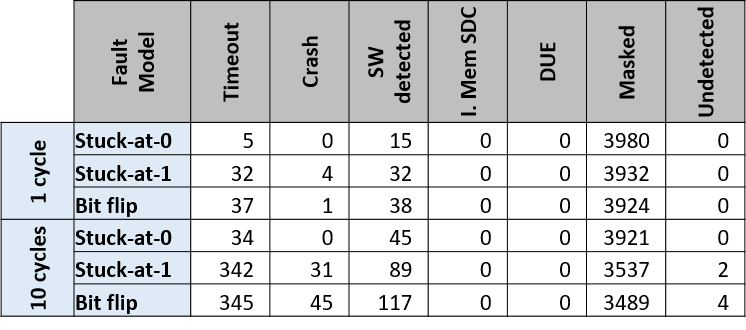
\includegraphics[width=1\columnwidth]{img/faultinjection2.png}
\end{table}
   

From all the simulations performed, the injected fault produced an error that the software comparison mechanism could not detect only in six. In all cases, the faults were injected in the write back stage. These errors led the system to a failure despite employing SafeDE to force a staggered execution. For that reason, we found it interesting to analyze those simulations in detail.


The benchmark FAC calculates the factorials from 0 to 12. Each result is accumulated in global variable. Finally, the value of this variable that contains the addition of all the factorials is compared to the expected result. FAC performs the factorial operation employing recursion. Figure \ref{fig:fac_assembly} shows the assembly code obtained after compiling the C code. We could distinguish three different sections: initialization, an outer loop that accumulates the factorial results and an inner loop that compute the factorials using recursion. 

In this particular case, the fault model is a bit flip that lasts 10 cycles. The bit selected to inject the fault is the least significant bit of the second write port of the register file, which flips to 1 and introduces an erroneous value in the write port. The fault is injected while the program is computing the factorial of 8. 

%%Rewrite it
However, those values are read through a bypass in the inner loop instead of from the register file, so no impact is observed in the inner loop. In the last iteration of the inner loop, the result of the factorial is stored in register a4 (line 8) with an erroneous value (due to the duration of the fault). Later, the register a4 is read as an operand for addw instruction in line 17, which accumulates all the calculated factorials. Therefore, this error is propagated to the output. Particularly, the erroneous result contains one bit flip in the least significant bit with respect to the correct result.

In the trail core, the fault is injected while the core is executing the outer loop. The fault affects several instructions, but all the errors except one are masked because they are either overwritten or not read since they are forwarded like in the head core. The error not masked is produced in line 17 when the result of the addition is written back to the a6 register, which stores the accumulation of the factorials. Again, the final value contains one bit flip with respect to the correct output in the least significant bit. Therefore, even though the fault affects both cores differently, in the end, it produces the same bit flip in the accumulated register (a6), which stores the output value.

Thus, the software is not capable of detecting the error, not because of a malfunctioning of SafeDE, but because of the semantics of the benchmark FAC. In fact, even if we used tight lockstepping, external core activity would be identical for both cores and no error would be detected. We content that, despite we could produce this apparent CCF in our fault injection campaign, such effect would be very unlikely to occur in practice since both cores have different states when the fault occurs, and this should lead to heterogeneous electric impact, hence causing heterogeneous errors (e.g., affecting only one core, or affecting different bits or locations of both cores).
%%%%%%%%%%%%

\begin{figure}[h]
    \centering
    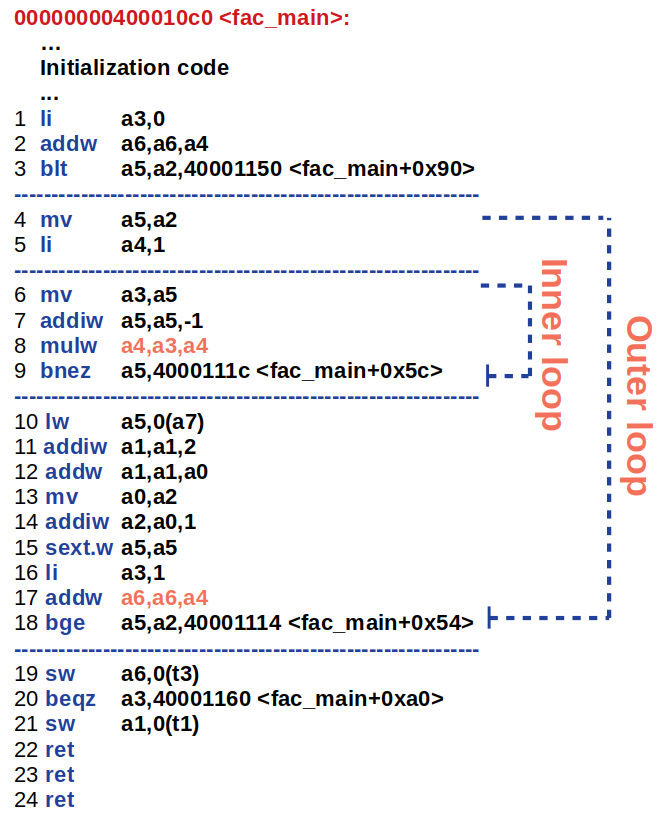
\includegraphics[scale=0.4]{img/fac_assembly.png}
    \caption{Excerpt of the assembly code of the benchmark FAC.} 
    \label{fig:fac_assembly}
\end{figure}

\bigskip



\subsection{Time Overhead}

To determine how much SafeDE afects the performance we have run the TACLe Benchmarks in three different scenarios:

\begin{enumerate}
    \item Isolation: Only one core executes the benchamrk while the other remains idle.
    \item Redundancy without diversity: Both cores execute the same benchmark without SafeDE enforcing any staggering. 
    \item Diverse Redundancy: Both cores run the same benchmark and SafeDE is active enforcing a staggering of 20 instructions ($Min\_TH_{stag}$ = 20)
\end{enumerate}

As stated before, it is convenient to set a staggering big enough to ensure that pipelines of both cores do not contain the same instruction in any of the pipeline stages at any point of the execution. Taking into account that NOEL-V cores are dual-issue with a 7-stages pipeline (pipelines can execute in parallel 14 instructions), 20 instructions of staggering (17 in practice) will suffice to avoid the two pipelines executing any common instruction. 

To generate two redundant processes, the same binary is loaded twice in different memory segments (one for each core). Each benchmark is executed 1,000 times to discard small variations across different executions due to random processes like the effect of the DRAM refresh in the memory latency. Although, the variation observed in the execution time between several executions of the same benchmarks has shown to be very low, in the order of a few tens of cycles.

Figure \ref{fig:tacle_results} shows the results. In the Figure, the execution time for redundancy without diversity and for diverse redundancy are normalized w.r.t the execution time in isolation. Results show that SafeDE computational overhead is really low. Namely, when SafeDE enforce diverse redundancy performance degrades by 0.3\% on average (up to 0.6\% for BITONIC) w.r.t executions in isolation, and 0.003\% (up to 0.6\% for IIR) on average w.r.t redundant executions without diversity. 

\begin{figure}[h]
    \centering
    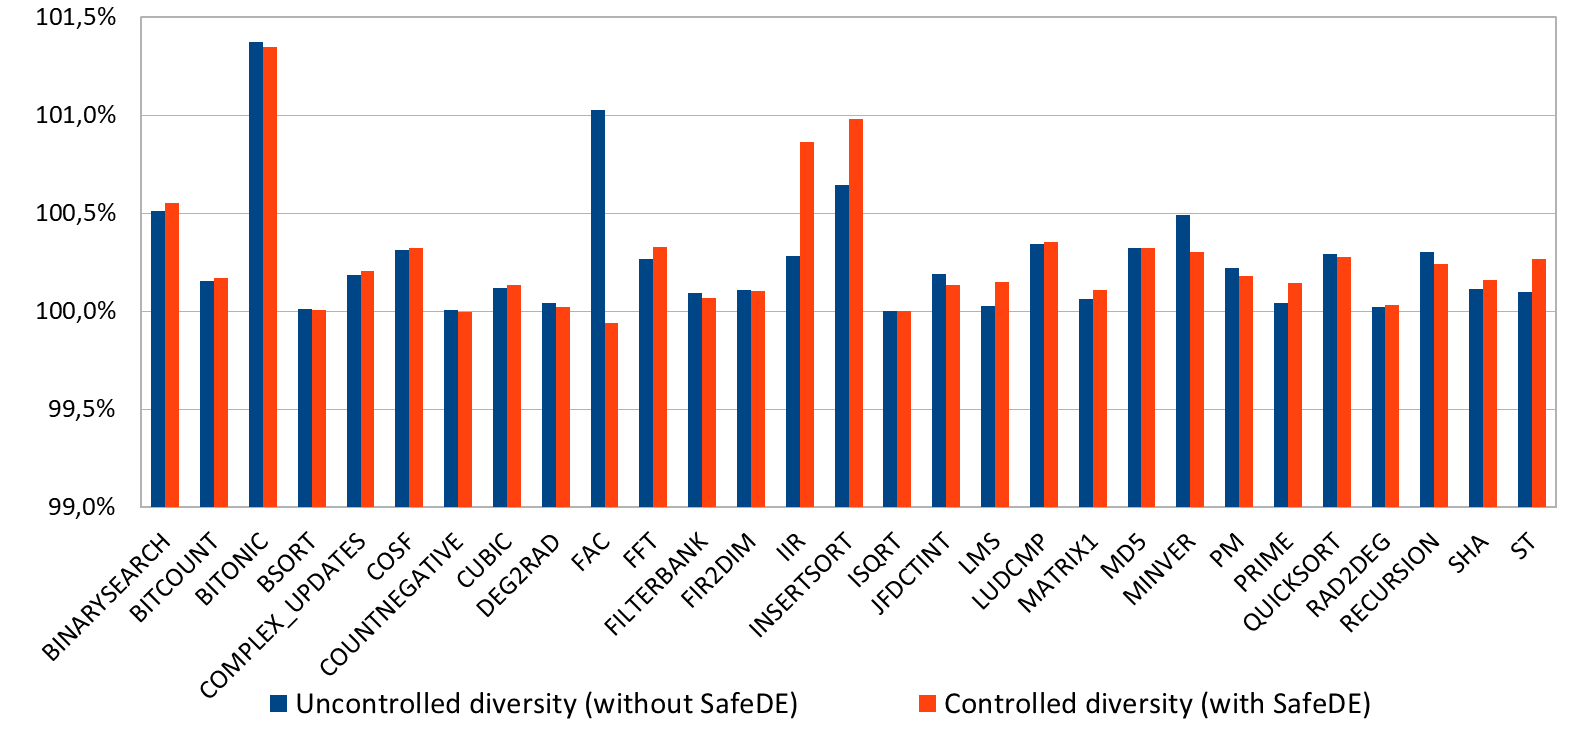
\includegraphics[scale=0.6]{img/tacle_results.png}
    \caption{Execution time of different TACLeBench benchmakrs normalized w.r.t. their execution time in isolation. Each benchmark is executed 1,000 times.}
    \label{fig:tacle_results}
\end{figure}


Results for Fac benchmark execution show that the execution time with controlled diversity is shorter than the execution time in isolation. To explain this anomalous result, we performed two simulations to compare the isolation run against the diverse redundancy execution. After a close examination, we found that the branch predictor was behaving differently, causing minor variations in both executions. These variations have a more significant impact in relative terms in smaller benchmarks like Fac, which executes only around 700 instructions. 

Summing up, execution time increase with diverse redundancy is negligible. SafeDE allows configuring small staggering thresholds, as we did in our evaluation (20 instructions), which are way below than those allowed by the software-only solution \cite{alcaide2020software}, positioning SafeDE as a much more efficient solution for light-weight lockstepped execution. 


\bigskip

\subsection{Hardware Costs}
\label{section:Hardware_resources}

We have employed the Vivado 2018.1 toolchain to synthesize and generate the bitstream targeting the Xilinx UlstraScale KCU105 Evaluation Kit featuring the Kintex XCKU040-2FFVA1156E FPGA. SafeDE implementation required 261 LUTs and 417 registers. Those numbers are really low compared with the resources required by each core (approximately 38,000 LUTs and 17,000 registers) or with the hardware resources required by the whole MPSoC (approximately 114,000 LUTs and 74,000 registers). Thus, SafeDE hardware costs are negligible. Namely, just 0.23\% of the LUTs and 0.56\% of the registers of the whole MPSoC are employed to implement SafeDE. Hardware overhead could be limited even more by removing the statistics registers which are only useful for debugging porpuses.


\bigskip




%%%% BDGET %%%
%\clearpage
%
%\section{Budget}
%{\selectlanguage{english}
%\foreignlanguage{english}{Depending on the thesis scope this document should include:}}

%%% ENVIRONMENT %%%
%\clearpage

%%% CONCLUSION AND FUTURE %%%
\clearpage
\section{Conclusions and future development: }

{This should include your summary, conclusions and recommendations. }

%%% BIBLIOGRAPHY %%%
\newpage

\medskip
\bibliographystyle{unsrt}
\bibliography{bibliography.bib}

%%% ANNEX %%%
\clearpage
\newpage

\begin{appendices}

{Appendices may be included in your thesis but it is not a requirement.}

\end{appendices}

\end{document}
